\documentclass[a4paper]{article} 

%中文环境设置
\usepackage{xeCJK} 
\usepackage{indentfirst}
\setlength{\parindent}{2em}
\usepackage{enumitem}

\usepackage{abstract}
\renewcommand{\abstractname}{摘要}
\providecommand{\keywords}[1]{\textbf{\textit{关键词}} #1}

\setCJKmainfont{STSong} % 中文主字体设置 

\usepackage[colorlinks,linkcolor=blue, citecolor=blue]{hyperref}

% 常用宏包
\usepackage{float}
\usepackage{stfloats}
\usepackage{graphicx}
\usepackage{color}
\usepackage{supertabular}

% 代码环境设置
\usepackage{listings}
\lstset{
	columns=fullflexible,
 	frame=single,
 	breaklines=true,
}
\definecolor{lightgray}{gray}{0.9}
\newcommand{\inlinecode}[2]{\colorbox{lightgray}{\lstinline[language=#1]$#2$}}

% 页面段落设置
\usepackage{multicol}
\usepackage{geometry}
\geometry{left=3.18cm, right=3.18cm, top=2.54cm, bottom=2.54cm}
\linespread{1.3}
%\setlength{\parskip}{0.5em} 

% 数学环境设置
\usepackage{amsmath}
\usepackage{amsthm}
\usepackage{amsfonts}
\newtheorem{myDef}{Definition} 
\newtheorem{myThm}{Theorem}
\newtheorem{myProp}{Property}

\begin{document} 
\title{矩阵特征值问题实验题}
\author{吴佳龙 2018013418}
\date{}
\maketitle

\begin{abstract}
	结合理论分析和编程计算,运用不同算法求解矩阵特征值和特征向量的数值解。运用的算法分别为经典Jacobi方法、Jacobi过关法、QR算法。
\end{abstract}

%\keywords{one, two, three, four}

\begin{multicols}{2}

\begin{section}{问题}

	计算以下三对角矩阵的特征值,要求达到三位有效数字。
	$$A=\left(\begin{array}{ccccc}{2} & {-1} & {} & {} & {} \\ {-1} & {2} & {-1} & {} & {} \\ {} & {\ddots} & {\ddots} & {\ddots} & {} \\ {} & {} & {-1} & {2} & {-1} \\ {} & {} & {} & {-1} & {2}\end{array}\right)$$
	
\end{section}

\begin{section}{Jacobi方法}

	\begin{subsection}{算法原理}
			
		对于实对称阵 $A$,记 $N(A)=\sum_{i \neq j}\left|a_{i j}\right|^{2}$,通过一系列 Givens 变换 $J(k,l;\theta)$,使 $N(A)$ 下降,最终收敛于对角阵,从而得到其所有特征值。
		
		其中,Givens 变换的参数 $k,l,\theta$ 的确定:令 $B = J^{-1}AJ$,则有 $$N(B) = N(A)+2\left|b_{k l}\right|^{2}-2\left|a_{k l}\right|^{2}$$,使得 $N(B)$ 尽量小,选取 $a_{kl}$ 为 $A$ 中非对角的绝对值最大的元素,并令 $b_{k l}=a_{k l} \cos 2 \theta+\frac{1}{2}\left(a_{l l}-a_{k k}\right) \sin 2 \theta=0$,解得 $$
			\{\begin{array}{l} { \text{if } a_{k k} \neq a_{l l} , \quad \tan {2\theta} = {2 a_{k l}\over a_{k k}-a_{l l}} } \\ {\text{if } a_{k k}=a_{l l} , \quad \cos 2 \theta=0 \Longrightarrow \theta={ \pi \over 4} } \end{array}$$
		
	\end{subsection}
		
	\begin{subsection}{算法描述}	
	
		\begin{subsubsection}{经典Jacobi方法}
			经典 Jacobi 方法的算法描述如下:
			
			记 $A^{(1)} = A$,选取 $\varepsilon$,对 $m=1,2,\dots$
			
			\begin{enumerate}
				\item 选取绝对值最大元素 $\left|a_{k l}^{(m)}\right|=\max _{i \neq j}\left|a_{i j}^{(m)}\right|$
				\item 若 $\left|a_{k l}^{(m)}\right|<\varepsilon $,则结束迭代;否则
				\item 确定 $J(k,l,\theta)$,做变换 $A^{(m+1)}=J A^{(m)} J^{-1}$
			\end{enumerate}
		\end{subsubsection}
		
		\begin{subsubsection}{Jacobi过关法}
		
			在扫描到为了提高扫描的效率,可采用 Jacobi 过关法,算法描述如下:
			
			确定一个阈值 $\delta_1 > 0$,例如 $\delta_1 = {\sqrt{N(A)}\over n}$,记 $m=1$ 并选取一个 $\varepsilon > 0$。
			
			\begin{enumerate}
				\item 循环扫描 $A$ 的所有非对角元,只要 $|a_{ij}|>\delta_m (i\neq j)$,就确定 $J(i,j,\theta)$,做相似变换 $JAJ^{-1}$。
				\item 直到 $A$ 的所有非对角元的绝对值都不超过 $\delta_m$,令 $\delta_{m+1} = \delta_m / n, m=m+1$
				\item 若 $\delta_m < \varepsilon$ 则退出。
			\end{enumerate}

			
			
		\end{subsubsection}
		
	\end{subsection}
		
	\begin{subsection}{收敛性分析}

		可以证明,在经典 Jacobi 算法中 $$ N(B)=N(A)-2\left|a_{k l}\right|^{2} \leq q \cdot N(A) $$ 其中 $q=1-\frac{2}{n(n-1)} \in[0,1)$。因此,$N\left(A^{(m+1)}\right) \leq q^{m} N(A) \rightarrow 0$,经典 Jacobi算法收敛。
		
	\end{subsection}
	
	\begin{subsection}{算法实现}
		
		经典 Jacobi 方法的 MATLAB 实现如下:
		
		\begin{lstlisting}[language=Matlab]
function [lambda, Q] = myJacobiClassic(A, eps)
% 经典Jacobi方法
% eps: 非对角元素绝对值小于eps,则终止
% lambda: 特征值
% Q: 对应特征值的特征向量
% 满足 inv(Q)*A*Q = diag(lambda)
[n,~] = size(A);
Q = eye(n);
while (true)
    C = abs(A - diag(diag(A)));
    val = max(max(C)); % 非对角元素的最大模
    if (val<eps)
        break
    end
    [k, l] = find(val==C); % 最大模的位置
    J = givensForJiacobi(A, k(1), l(1));
    A = J*A*J';
    Q = Q*J';
end
lambda = diag(A);    
end
		\end{lstlisting}
		
		Jacobi 过关法的 MATLAB 实现如下:
		
		\begin{lstlisting}[language=Matlab]
function [lambda, Q] = myJacobiThreshold(A, eps)
% Jacobi过关算法
% eps: 过关法阈值小于eps,则终止
% lambda: 特征值
% Q: 对应特征值的特征向量
% 满足 inv(Q)*A*Q = diag(lambda)
[n,~] = size(A);
Q = eye(n);
% 初始阈值 sqrt(N(A))/2
delta = sqrt(sum(sum(abs(A)))-sum(sum(diag(abs(A)))))/n;
while (delta>eps)
    while (true)
        mapped = false;
        % 过关扫描
        for i = 1:n
            for j = i+1:n
                if (abs(A(i,j))>delta)
                    % givens 变换
                    J = givensForJiacobi(A, i, j);
                    A = J*A*J';
                    Q = Q*J';
                    mapped = true;
                end
            end
        end
        % 所有元素都绝对值小于阈值
        if (~mapped)
            break
        end
    end
    delta = delta/n;
end
lambda = diag(A);    
end
		\end{lstlisting}	
		
		其中,求解 Givens 变换矩阵的函数实现如下:
		
		\begin{lstlisting}[language=Matlab]
function [J] = givensForJacobi(A,k_,l_)
% Jacobi方法中的givens变换矩阵
k = min(k_,l_); l = max(k_,l_);
[n,~] = size(A);
if (A(k,k) ~= A(l,l))
    ct2 = (A(k,k)-A(l,l))/2/A(k,l);
    t = sign(ct2)/(abs(ct2) + sqrt(1+ct2^2));
    c = 1/sqrt(1+t^2); s = c*t;
else
    c = cos(pi/4); s = sin(pi/4);
end
J = eye(n);
J(k,k) = c; J(l,l) = c;
J(k,l) = s; J(l,k) = -s;
end
		\end{lstlisting}	
		
	\end{subsection}
	
	\begin{subsection}{计算结果}
	
		\begin{subsubsection}{经典 Jacobi 方法}
		
			对于不同的 $n$,调用函数 \inlinecode{Matlab}{myJacobiClassic(A, 1e-7)},并观察计算时间和计算结果的精度。
		
			其中,当 $n=3$ 时,由 MATLAB 内置 \inlinecode{Matlab}{eig} 函数给出特征值 $$0.585786437626905$$$$2.000000000000000$$$$3.414213562373095$$ 由实现的经典 Jacobi 方法计算得特征值为 $$0.585786437626905$$$$3.414213562373095$$$$2.000000000000000$$ 对应的特征向量构成的矩阵 
			$$\left(
				\begin{matrix}
				0.5000 & -0.5000 & -0.7071 \\
   				0.7071 &  0.7071 &  0.0000 \\
    			0.5000 & -0.5000 &  0.7071
				\end{matrix}
			\right)$$
			
			计算结果符合实际,且具有较高的精度。
			
			选取更多 $n$ 后,给出结果如下:
			
			\begin{table}[H]
			\begin{tabular}{c|c|c}
			\hline
			       & 特征值有效位数 & 计算时间(s)  \\ \hline
			$n=3$  & 15位     & 0.000358 \\
			$n=5$  & 14位     & 0.000821 \\
			$n=10$ & 13位     & 0.003996 \\
			$n=15$ & 13位     & 0.008564 \\ \hline
			\end{tabular}
			\end{table}
			
		\end{subsubsection}

		\begin{subsubsection}{Jacobi 过关法}
		
			对于不同的 $n$,调用函数 \inlinecode{Matlab}{myJacobiThreshold(A, 1e-7)},并观察计算时间和计算结果的精度。
			
			计算结果基本与经典 Jacobi 方法一致,具体如下:
			
			\begin{table}[H]
			\begin{tabular}{c|c|c}
			\hline
			       & 特征值有效位数 & 计算时间(s)  \\ \hline
			$n=3$  & 14位     & 0.000244 \\
			$n=5$  & 15位     & 0.000442 \\
			$n=10$ & 13位     & 0.004956 \\
			$n=15$ & 12位     & 0.002785 \\ \hline
			\end{tabular}
			\end{table}
			
		\end{subsubsection}

	\end{subsection}

\end{section}


\begin{section}{QR算法}

	\begin{subsection}{算法原理}
		
		对于 $\forall A \in \mathbb{C}^{n \times n}$,可对 $A$,进行 QR 分解 $A=QR$。记 $B=RQ$ ,则有 $B = Q^HAQ$ 与 $A$ 相似。
		
		由此,QR算法的算法描述如下:令 $A_1 = A$,对 $k=1,2,\dots$
		
		\begin{itemize}
			\item 分解 $A_k = Q_k R_k$
			\item 令 $A_{k+1} = R_k Q_k, k=k+1$
			\item 若 $A_k$ 的非对角元素绝对值小于阈值,则结束
		\end{itemize}
		
		对于 QR 算法的收敛性有如下定理:
		
		\begin{myThm}
			
			设 $A \in \mathbb{R}^{n \times n}$,特征值分别为 $|\lambda_1| > \cdots > |\lambda_n| >0$,对应的特征向量为 $x^{(i)}$,记 $X = [x^(	1), \cdots, x^(n)]$ 并设存在LU分解 $X^{-1}=LU$,则 QR 算法产生的 $\left\{A_{k}\right\}_{k=1}^{+\infty}$ 基本收敛到上三角阵  $$\lim _{k \rightarrow+\infty} a_{i i}^{(k)}=\lambda_{i}, i=1, \cdots, n$$
			 	
		\end{myThm}
		
		\begin{subsubsection}{上 Hessenberg 矩阵}
		
			利用 Household 变换或者 Givens 变换都能将矩阵相似变换为上 Hessenberg 矩阵。 
		
			在 QR 算法中,若先将 $A$ 相似变换到上 Hessenberg 矩阵 $H$,则可以证明在 QR 算法的过程中 $A_k$ 的形式保持为上 Hessenberg 矩阵不变,这可以减少算法的运算量,提高效率。
			
		\end{subsubsection}
				
	\end{subsection}
	
	
	\begin{subsection}{算法实现}
	
		QR算法的 MATLAB 实现如下:
		
		\begin{lstlisting}[language=Matlab]
function [lambda, X] = myQR(A, eps)
% QR算法求解特征值
% eps: 下对角元素绝对值小于eps,则终止
% lambda: 特征值
% X: 对应特征值的特征向量
% 满足 inv(X)*A*X = diag(lambda)
[n,~] = size(A);
% 为了减少运算量,可将A先转化为上Hessenberg阵
% 在本次作业中 A 已经为该形式
% H = toHessenberg(A);
H = A;
while (max(max( tril( abs( H-diag(diag(H)) )) ))>eps)
    [U,R] = QRForHessenberg(H);
    H = R*U;
end
lambda = diag(H);
% 特征向量可用反幂法求得
X = zeros(n,n);
for i=1:n
    [lambda(i), X(:,i)] = inversePowerMethod(A, lambda(i)+(1e-5*randn()), eps);
end
end
		\end{lstlisting}
		
		其中,利用 Givens 变换对上 Hessenberg 矩阵进行QR分解的实现如下:
		
		\begin{lstlisting}[language=Matlab]
function [U, R] = QRForHessenberg(H)
% 上Hessenberg矩阵的QR分解
% 结果满足 H = UR
[n,~] = size(H);
Ut = eye(n);
for i=1:n-1
    t = H(i+1,i)/H(i,i);
    c = 1/sqrt(1+t^2);
    s = t*c;
    % givens 变换
    H(i,:) = H(i,:)*c + H(i+1,:)*s;
    H(i+1,:) = (c+s^2/c)*H(i+1,:) - s/c*H(i,:);
    Ut(i,:) = Ut(i,:)*c + Ut(i+1,:)*s;
    Ut(i+1,:) = (c+s^2/c)*Ut(i+1,:) - s/c*Ut(i,:);
end
U = Ut';
R = H;
end
		\end{lstlisting}	
		
		反幂法实现如下:
		
		\begin{lstlisting}[language=Matlab]
function [lambda, v] = inversePowerMethod(A, q, eps)
% 原点位移的反幂法求解特征值和特征向量
% eps: 相邻两次迭代结果小于eps,则终止
[n,~] = size(A);
A = A-q*eye(n);
v = ones(n, 1);
k=0;
while (true)
    k = k+1;
    z = A\v;
    [~,pos] = max(abs(z));
    m = z(pos); % 最大模元素
    v = z/m;
    if (k>1 && abs(1/m-1/last_m)<eps) 
        break;
    end
    last_m = m;
end
lambda = 1/m+q;
end		
		\end{lstlisting}	

	\end{subsection}
	
	\begin{subsection}{计算结果}
	
		对于不同的 $n$,调用函数 \inlinecode{Matlab}{myQR(A, 1e-7)},并观察计算时间和计算结果的精度。
			
		计算结果基本与 Jacobi 方法一致,具体如下:
			
		\begin{table}[H]
		\begin{tabular}{c|c|c}
		\hline
		       & 特征值有效位数 & 计算时间(s)  \\ \hline
		$n=3$  & 5位     & 0.000691 \\
		$n=5$  & 5位     & 0.001453 \\
		$n=10$ & 5位     & 0.006394 \\
		$n=15$ & 5位     & 0.020118 \\ \hline
		\end{tabular}
		\end{table}
				
	\end{subsection}
	
\end{section}

\begin{section}{方法比较}
	选取不同的 $n$, 分别调用 \inlinecode{Matlab}{myQR(A, 1e-7)} \inlinecode{Matlab}{myJacobiClassic(A, 1e-7)} \inlinecode{Matlab}{myJacobiThreshold(A, 1e-7)} ,比较以上三种方法的计算时间,结果如图 \ref{cp_time} 所示。
	
	\begin{figure*}[ht] %h默认参数是可以浮动,不是固定在当前位置。如果要不浮动,你就可以使用大写float宏包的H参数,固定图片在当前位置,禁止浮动。
		\centering %使图片居中显示
		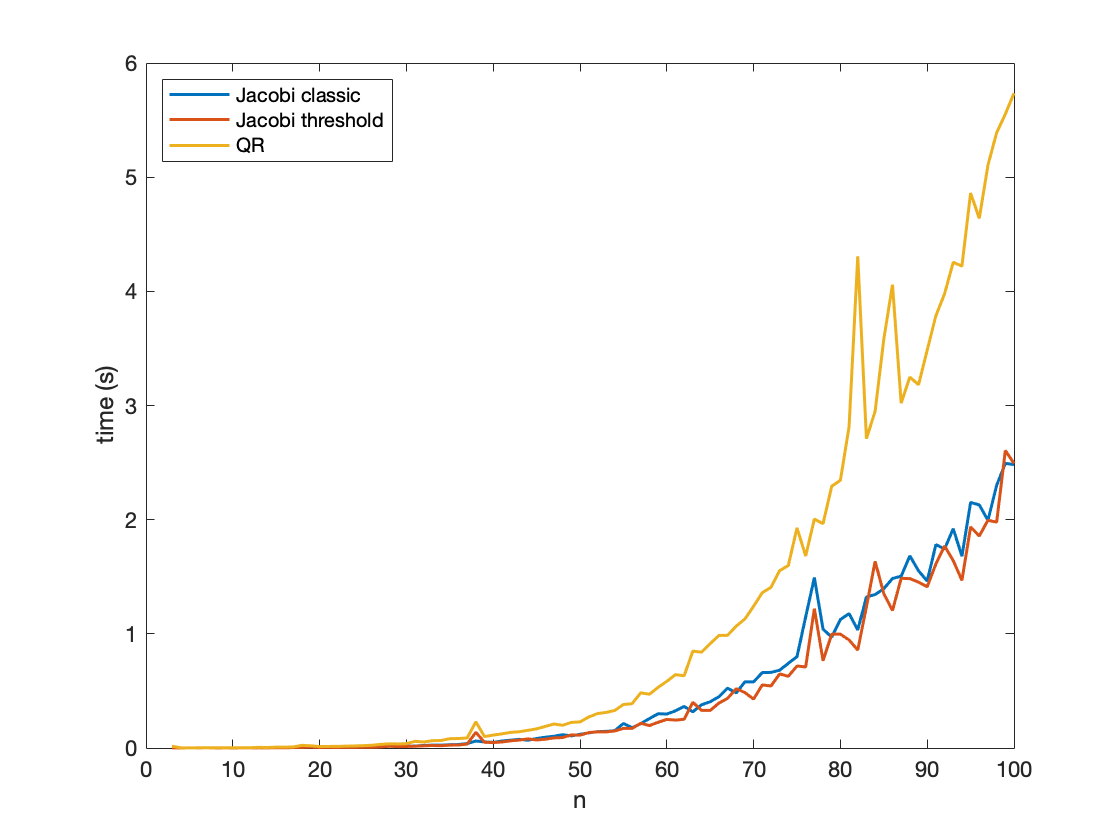
\includegraphics[width = \textwidth]{img/compare_time.png} 
		\caption{不同算法的计算时间}
		\label{cp_time} 
	\end{figure*}	
	
	可以看到,在本次实验中,QR 算法的效率慢于 Jacobi 方法,这与实验中的 $A$ 接近对角阵的性质有很大关系;且 Jacobi 过关法整体上快于经典 Jacobi 方法,符合过关法的初衷,但差异并不显著。
	
	另外,还发现,针对上 Hessenberg 矩阵的性质利用 Givens 变换或 Household 变换进行的 QR 分解能大大降低运算量,提高 QR 算法的计算效率。
	
\end{section}

\begin{section}{总结}
	
	本次实验对于几种不同的求解特征值问题的算法进行了理论分析和编程计算,结果符合预期,实现的算法具有较快的效率和较高的精度。
	
	另外,还对几种方法的运行效率进行了比较探究,得出了 Jacobi 过关法稍快于经典 Jacobi 方法,以及上 Hessenberg 阵的形式能有效提升 QR 算法的计算效率等结论。
	
\end{section}

\end{multicols}



%\bibliographystyle{unsrt}
%\bibliography{ref.bib}

%\begin{thebibliography}{99}    %参考文献开始
%	\bibitem{ml}周志华. 机器学习[M]. 清华大学出版社, 2016.   
%\end{thebibliography}	

\end{document}

